\begin{figure}[h!]
	\begin{center}
		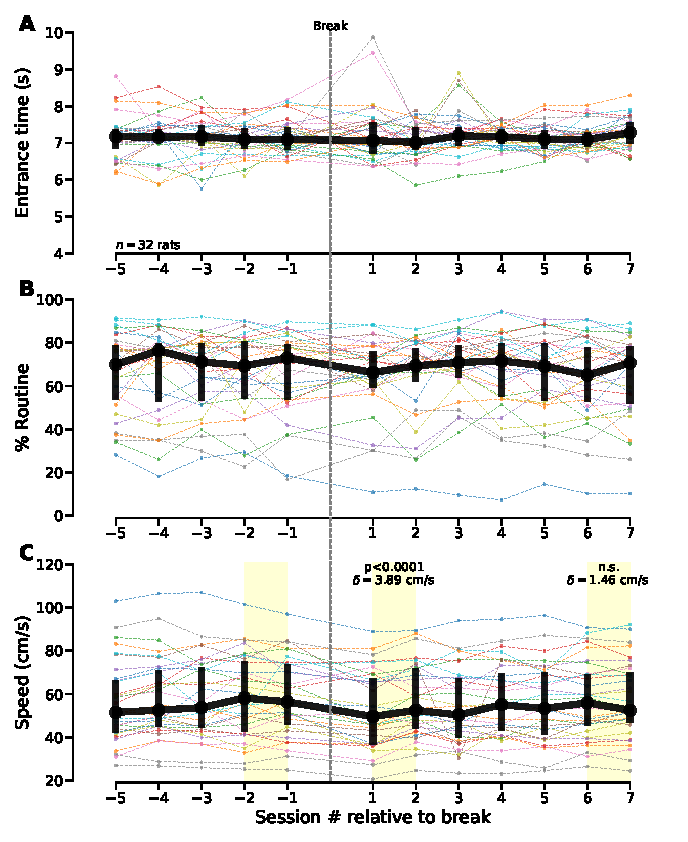
\includegraphics[scale=1]{ch-appendicies/figures/BreakEffect.pdf}
		\caption[Impact of a Two-week Break]
		{\textbf{Impact of a two weeks break in practice on performance.}
		\textbf{A-C)} Task performance before and after a two weeks-long break in practice.
		Non-lesioned animals had stable performance before the two weeks-long break (same duration than lesion recovery period) in practice.
		\textbf{A)} Entrance time.
		\textbf{B)} Percentage of trials during which animals used the wait-and-run routine.
		\textbf{C)} Speed of the animals when they ran toward the reward area.
		A small but significant reduction in running speed was observed just after the break ($\delta$ denotes the effect size).
		}
		\label{fig:appendix:break}
	\end{center}
\end{figure}